% % % % % % % % % % % % % % % % % % % % % % % % % % % % % % % % % % % %
\documentclass[english]{article}
\usepackage[T1]{fontenc}
\usepackage[latin9]{inputenc}
\usepackage{fancyhdr}
\pagestyle{fancy}
\usepackage{textcomp}
\usepackage{babel}
\usepackage{url}
\usepackage{color,soul}
\usepackage{graphicx}
\usepackage[pdftitle={Adaptable Replication Based on Ant Algorith},%
		hidelinks,colorlinks=true, linkcolor=black, citecolor=cyan, filecolor=green, urlcolor=blue]{hyperref}
\usepackage{mathtools}
\usepackage{amssymb}
\usepackage[numbers]{natbib}
%\usepackage{glossaries}
%\usepackage[xindy]{glossaries}

%\makeglossaries

% % % % % % % % % % % % % % % % % % % % % % % % % %
% Aconyms for SyncFree project.
%
% Author: Amadeo Asco
% Last updated: 24 July 2014
% % % % % % % % % % % % % % % % % % % % % % % % % %
% The acronym package helps you manage acronyms and acronym lists in your documents, http://www.mackichan.com/index.html?techtalk/456.htm~mainFrame
% for the glossary to show up in Table of Contents you need to additionally add toc option
\usepackage[toc,nonumberlist]{glossaries}
%\showthe\hsize% interrupts latex and shows value of \hsize
\setlength{\glsdescwidth}{0.82\hsize}%
% to remove extra line between groups
\renewcommand{\glsgroupskip}{}
% To get rid of the full stop after the description in the glossary
\renewcommand{\glspostdescription}{}
\makeglossaries

% Start definitions ---------------------------
% Add all of the definitions for the abbreviations
\newacronym{2i}{2i}{Secondary Indexing}
\newacronym{2pset}{2P-Set}{Two-Phase Set}
\newacronym{acid}{ACID}{Atomicity, Consistency, Isolation, Durability}
\newacronym{b2b}{B2B}{Business to Business}
\newacronym{base}{BASE}{basically available, soft state, eventual consistency}
\newacronym{cci}{CCI}{Causality, Convergence and Intention}
\newacronym{cmrdt}{CmRDT}{Op-based Convergent Replicated Data Type}
\newacronym{cprdt}{CPRDT}{Conflict-free Partially Replicated Data Type}
\newacronym{crdt}{CRDT}{Conflict-free Replicated Data Type}
\newacronym{cqrs}{CQRS}{Command Query Responsibility Segregation}
\newacronym{cvrdt}{CvRDT}{State-based Convergent Replicated Data Type}
\newacronym{dc}{DC}{Data Centre}
\newacronym{ec}{EC}{Eventual Consistency}
\newacronym{ga}{GA}{Genetic Algorithm}
\newacronym{gset}{G-set}{State-based increment-only Counter}
\newacronym{gp}{GP}{General Practitioner}
\newacronym{ha}{HA}{High Availability}
\newacronym{id}{ID}{identifier}
\newacronym{lww}{LWW}{Last-Writer-Wins}
\newacronym{lwwr}{LWW-Register}{Last-Writer-Wins Register}
\newacronym{mdc}{MDC}{Multi Data Centre}
\newacronym{mv}{MV}{Multi-Valued}
\newacronym{mvr}{MV-Register}{Multi-Valued Register}
\newacronym{orset}{OR-set}{Observed-Removed Set}
\newacronym{rdbms}{RDBMS}{Relational Database Management System}
\newacronym{rga}{RGA}{Replicated Growing Array}
\newacronym{rest}{REST}{Representational State Transfer}
\newacronym{rpc}{RPC}{Remote Procedure Call}
\newacronym{cap}{CAP}{Consistency, Availability and Partition tolerance}
\newacronym{sec}{SEC}{Strong Eventual Consistency}
\newacronym{ttl}{TTL}{Time To Live}
\newacronym{uset}{U-Set}{Two-Phase Set with unique elements}
\newacronym{wp1}{WP1}{Work Package 1}
\newacronym{wp2}{WP2}{Work Package 2}
\newacronym{wp3}{WP3}{Work Package 3}
\newacronym{wp4}{WP4}{Work Package 4}
\newacronym{wp5}{WP5}{Work Package 5}
% end abbreviations ---------------------------

%\ifnum\showDefinitions=1
% Add all of the definitions
%\newglossaryentry{bwd}{name={box-and-whisker diagram}, text={box-and-whisker diagram}, first={box-and-whisker diagram},
%    description={\parbox{10.6cm}{\medskip The bottom and top of the box are the 25th and 75th percentile (the lower and upper quartiles, respectively), and the band near the middle of the box is the median, whereas the dot represent the mean. The ends of the whiskers represent the minimum and maximum of all of the data.\medskip}}}
% end definitions -----------------------------
%\fi

\glsdisablehyper


\begin{document}

\title{Adaptable Replication Based on Ant Algorithm}

\author{Amadeo Asc\'{o}}

\date{24$^{th}$ September 2014}

\maketitle

%{\bf Keywords}: Adaptive Replication, SyncFree


\section{Introduction}
	The amount of data being processed in \glspl{dc} keeps growing at enormous rate \cite{Hey2009a, Cisco2014a, Chanthadavong2014a}. Some of the areas where the amount of stored data already reach \glspl{tb} and even \glspl{pb} are data mining, particle physics, climate modelling, high energy physics and astrophysics, to site few, data which needs to be shared and analysed \cite{KingsyGrace2014a, MohdZin2012a, Naseera2009a}. \glspl{dc} are able to ensure that stored data is highly accessible and scalable. But the location of a \gls{dc} in respect of the client accessing the data has an impact on availability, access times (latency - accessibility) and costs derived from providing the data. Replicating some of the data at multiple sites is a possible solution to reduce some of these undesirable effects, \cite{Briquemont2014a, Abad2011a, Venugopal2006a}. An increase in the number of replications may result in a large bandwidth savings and lead to a reduction in user response time on reads. But keeping too many replicas of the data incurs in extra costs, such as extra replication traffic to keep all versions of the data coherent (writes), extra required storage and extra computational power \cite{Goel2006a}.
	
	This means that finding an optimal replication distribution that minimises the amount of network traffic given certain read and write frequencies for various objects should alleviate these extra costs when replicating, \cite{Wolfson1990a, Briquemont2014a}. Given the volume of operations considered, which are predominately higher in reads than writes, and the speed of the access expected then any algorithm suitable to be applied to this constrain optimisation problem must have a very fast execution time.

	The replications may be grouped into two types; {\bf static replication} where a replica persist until it is deleted by a user or its duration expires, and {\bf dynamic replication} where the creation and deletion of a replica are managed automatically and normally directed by the access pattern of the data used by the users \cite{Dong2008a}. In static replication the major drawback is their inability to adapt to changes in the access pattern of the data used by the users.
	
	The proposed algorithm is base on Wolfson's algorithm, \cite{Wolfson1990a}, which proposes an adaptive algorithm for replicated data between processors which takes into account the changes in the read-write pattern of the processors in the network. Also the proposed algorithm is based on the principles of the Ant Colony Optimisation algorithms, which are inspired in the behaviour of ant colonies when deciding which path to follow when foraging, \cite{dorigo1992a}.
	
	It should be noted that the main propose of the replication is not to recover from disasters as this is the responsibility of the recovery centres which are data centres sufficiently close to the operational \gls{dc}, they are associated to, so copies can be processed quickly enough but at the same time sufficiently far apart as to avoid any potential geographical issues that may happen to the \glspl{dc}, i.e. earthquakes, fire that destroys the \gls{dc}, the shutting down of main power plant which provides energy to the \gls{dc}. Neither it is the \gls{dc} responsibility to provide analytical services as these are provided by the data warehouse(s). The main propose of the considered \glspl{dc} is to provide operational access to clients (operational \glspl{dc}), which corresponds to intensive read/write operations to the client's most recent data. The following references to \glspl{dc} in this document referrer to operational data centres.


\section{Algorithm}
The general idea of this algorithm is to decide without the need of human intervention where and when to replicate with the main objective of reducing the latency and network traffic (reduce usage of bandwidth).

In general terms any read operation in a \gls{dc} reinforces the need for a replica of the data in such \gls{dc}, similarly but perhaps with a different degree it happens with the write operations, but write operations decrease the need for a replica of the data in the other \glspl{dc} with replicas of the data, so eventually these \glspl{dc} will not have any replica of the data. Given that we do not want to keep replicas if it is not necessary then the need for such replica will decay as time pass, but always making sure that the data is present (replicated) at least in one of the \glspl{dc}. This algorithm is further explained below together with a mathematical representation. The variables and constants used in the algorithm are summarised in Table \ref{tbl:vars_consts}.
\begin{table}[ht]
	\begin{tabular}{ |l|p{7.8cm}|l|}
		\hline
		{\bf Variable}    & {\bf Description} & {\bf Type} \\
		\hline
		\hline
		$DC$                & It is the set of all \glspl{dc}. $d$ identifies one of the \glspl{dc}, $d \in \{1,\dots, |DC|\}$. \gls{dc}$_{d}$ represents the \gls{dc} $d$ which holds some data, D$_{d}$. &  $d \in \mathbb{N}^{+}$ \\
		\hline
		$D_{kd}$           & It represents the replica of data $k$ in \gls{dc} $d$, $k \in \{1,\dots, |D|\}$. & $k \in \mathbb{N}^{+}$ \\
		\hline
		$r_{kd}$            & It is the number of reads for data $k$ requested on \gls{dc} $d$. & $r_{kd} \in \mathbb{N}_{0}$ \\
		\hline
		$\Delta r_{k}$   & It represents the strengthening of the replication in the \gls{dc} used to execute one read. & $\Delta r_{k} \in \mathbb{R}^{+}$ \\
		\hline
		$w_{kd}$           & It is the number of writes for data $k$ directly requested on \gls{dc} $d$. & $w_{kd}\in \mathbb{N}_{0}$ \\
		\hline
		$\Delta w_{k}$  & It represents the strengthening of the replication in the \gls{dc} directly used to execute a write. & $\Delta w_{k} \in \mathbb{R}^{+}$ \\
		\hline
		$w_{kdi}$          & It represents the decay of the replication in the \gls{dc} $i$ consequence of the write request in \gls{dc} $d$. This value will depend of both \glspl{dc} $d$ and $i$ and may also depend on the time of the day or other useful information available at the time it is used. & $w_{kdi} \in \mathbb{R}^{+}$ \\
		\hline
		$T_{k}$             & It is the replication strength required to start the replication of data $k$ in a \gls{dc} which does not currently contain a replica of the data. & $T_{k} \in \mathbb{R}^{+}$ \\
		\hline
		$\Gamma$      & It is the decay of the replication strength with time. A simple example corresponds to a constant decay ($\tau$) of the replication strength from the time the replica was created, $\Gamma = \Delta t * \tau$. & $\Gamma \in \mathbb{R}^{+}$ \\
		\hline
		$R_{k}$            & It is the number of replicas for data $k$, $D_{k}$. & $R_{k} \in \mathbb{N}_{0}$ \\
		\hline
		$M_{k}$           & Minimum number of replicas of data k, default $M_{k} = 1$. & $M_{k} \in \mathbb{N}_{0}$ \\
		\hline
		$F_{k}$            & The replication strength for data $k$, $F_{k} \le L_{k}$. & $F_{k} \in \mathbb{R}_{0}$ \\
		\hline
		$L_{k}$            & The maximum replication strength for data $k$, $F_{k} \le L_{k}$. & $L_{k} \in \mathbb{R}_{0}$ \\
		\hline
	\end{tabular}
	
	\caption{List of variables and constants.}
	\label{tbl:vars_consts}
\end{table}

Equation \ref{eq:data_replicated} represents the existence of a replica of data $k$ in \gls{dc} $d$, $c_{dk} = 1$, or its absence $c_{dk} = 0$. $R_{k}$ is the number of replicas of data $k$, as expressed in Equation \ref{eq:num_replicas}.
\begin{equation} \label{eq:data_replicated}
	c_{dk} = \left\{
		\begin{array}{ll}
			1 & if D_{k} \in DC_{d} \text{ } (\exists D_{kd})\\
			0 & otherwise
		\end{array}
	\right.
\end{equation}

\begin{equation} \label{eq:num_replicas}
R_{k} = \sum^{|DC|}_{d = 1} c_{dk}
\end{equation}

$F_{kd}$ represents the full strength of the replication of the data $k$ in \gls{dc} $d$, which it is expressed in Equation \ref{eq:replication_strength}.
\begin{equation}  \label{eq:replication_strength}
	 F_{kd} = \min(r_{kd} * \Delta r_{k} + w_{kd} * \Delta w_{k} - \sum^{|DC|}_{i = 1, i \neq d} w_{kd} * \Delta w_{kdi} - c_{kd} * \Gamma, L_{k})
\end{equation}

%\begin{equation}  \label{eq:inter_dc_decay}
%	\Delta w_{kdi} = 0 \textbf{ } \forall d = i \text{ or } c_{kd} = 0 \text{, or } c_{ki} = 0
%\end{equation}

Equation \ref{eq:replication_strength} shows that the replication strength for the data $k$ in \gls{dc} $d$ is strengthened by the reads and writes requested through \gls{dc} $d$, with intensities $\Delta r_{k}$ and $\Delta w_{k}$ respectively, and weakened  by the writes requested through other \glspl{dc} than \gls{dc} $d$, with intensity $\Delta w_{kdi}$, and it is furthermore weakened by a temporal decay on the replication strength (last term in the equation). Where Equation \ref{eq:replication_strength} states that only \glspl{dc} with a replica of the data, $D_{k}$, will be penalised by writes and time, which in practice it is achieved by not sending the write to those \glspl{dc} so it does not incurred in any extra cost when implementing it. Similarly $\Gamma$ will not be applied to \glspl{dc} without replicas of the data with the exceptions of those candidate \glspl{dc} where the data may later be replicated. Reads may increase the number of replicas where writes may strengthen the replication in a \gls{dc} but may also potentially remove a replica from one of the other \glspl{dc}, effect that it is strengthen by the temporal decay of the replication strength.

$T_{k}$ is the threshold of the replication strength of data $k$ which determine when to keep an existing replica in a \gls{dc}, as expressed in Equation \ref{eq:replicas_threshold}.
\begin{equation} \label{eq:replicas_threshold}
	\exists D_{kd} \text{, } t_{0} \text{ } (D_{kd} \in DC_{d}) \text{ if } F_{kd} \le T_{k} \text{ } \text{ and } \nexists D_{kd} \text{, } t < t_{0}  \text{ and } F_{kd} > T_{k} \text{, } t_{0}
\end{equation}

The Equations \ref{eq:no_replica} and \ref{eq:no_replica1} show the cases where a data $k$ is not replicated in a \gls{dc} $d$.  A replica in a \gls{dc}, with no replication strength, will only be destroyed if the number of replicas is bigger than a minimum, $M_{k}$, also for a \gls{dc} which does not have a replica of the data the replication strength must be higher than a pre-set threshold $T_{k}$ to create a new replica, as represented in Equation \ref{eq:replicas_threshold}.
\begin{equation} \label{eq:no_replica}
\nexists D_{kd} \text{, } t > t_{0} \text{ if } \exists D_{kd} \text{ for } t < t_{0} \text{ and } F_{kd} \le 0 \text{, } R_{k} > M_{k} \text{, } t_{0}
\end{equation}

\begin{equation} \label{eq:no_replica1}
	\nexists D_{kd} \text{, } t_{0} \text{ if } \nexists D_{kd} \text{, } t' \le t_{0} \text{ and } F_{kd} \le T_{k} \text{, }  t_{0}
\end{equation}

Each \gls{dc} with a replica of the data must know about the other \glspl{dc} that have replicas of the same data in order to manage the replication of such data.

If data $k$ is only replicated in one \gls{dc} $d$ and a write is requested using a different \gls{dc} $j$ than the one it is correctly replicated in, so that its replication strength in \gls{dc} $d$ is reduced to zero or under ($F_{kd} < 0$), then the data will continue to be replicated in that \gls{dc} until a replica is place in another \gls{dc} or its replication is increased over zero.

For the time being, it is considered the case where $w_{kdi}$ increases with the distance (network distance) between both \glspl{dc} $d$ and $i$. Also it is assumed that the value is symmetrical, such that $w_{kdi} = w_{kid}$, so there is the same cost of transferring the data from \gls{dc} $d$ to \gls{dc} $i$ than from \gls{dc} $i$ to \gls{dc} $d$. If to transfer the data between both \glspl{dc} $d$ and $i$ requires the use of an intermediate \gls{dc} $j$ then $w_{kdi} \ge w_{kdj} + w_{kji}$, similarly if many intermediate nodes are used the decay will be at least the sum of the intermediate decays.

The effect of $\Gamma$ is required to ensure that in absence of writes some replications will still vanish and if the reads are concentrated in a few \glspl{dc} then the replicas in other \glspl{dc} will be eventually removed. There is an extra requirement in the case that the data only exists in a \gls{dc}, in which case, the temporal effect should be ignored, so the data exists at least in one \gls{dc}.

A read request to a \gls{dc}, which does not have a replica of the data, will be forwarded to the closest \gls{dc} with a replica. The \gls{dc} with a replica will not gain strength from this read operation as the read was not initiated directly from itself. This \gls{dc} will then have a knowledge of the data but not a replica, so this knowledge will be used in subsequent reads/writes to the \gls{dc} which eventually may keep a replica. Once the replication strength is higher than the threshold ($T_{k}$), this \gls{dc} will notify all the \glspl{dc} with a replica of the existence of the new \gls{dc} with a replica.

It may also be required to use another temporal effect the \gls{ttl} to make sure that eventually the data will be fully removed. This value may not be applied to data stored in recovery centres and data warehouses which may have their own \gls{ttl}. Also it would be desirable for data that expires to be copied into those data centres before it is removed from all the \glspl{dc}.

Overall it is assumed that reads and writes are not treated differently, so they are not directed to different \glspl{dc}, otherwise it may be needed some adjustment to the approach presented here or may even invalidate it.

The algorithm is optimal in the sense that when the replication scheme stabilises, the total number of replicas required for the reads and writes is minimal.

The read sequence diagrams for this algorithm are shown in Table \ref{tb:read_sequence_diagrams} with its flowchart presented in Figure \ref{fig:read_flowchart}, and the write ones are shown in Table \ref{tb:write_sequence_diagrams} with its flowchart presented in Figure \ref{fig:write_flowchart}. The second figure in Table \ref{tb:read_sequence_diagrams} may also have a notification for all \glspl{dc} with a replica of the data to notify of the new replica which will be sent by the direct \gls{dc} for when the threshold has been passed and a replica is created in the direct \gls{dc}.
\begin{table}[ht!]
	\begin{center}
		\begin{tabular}{c}
			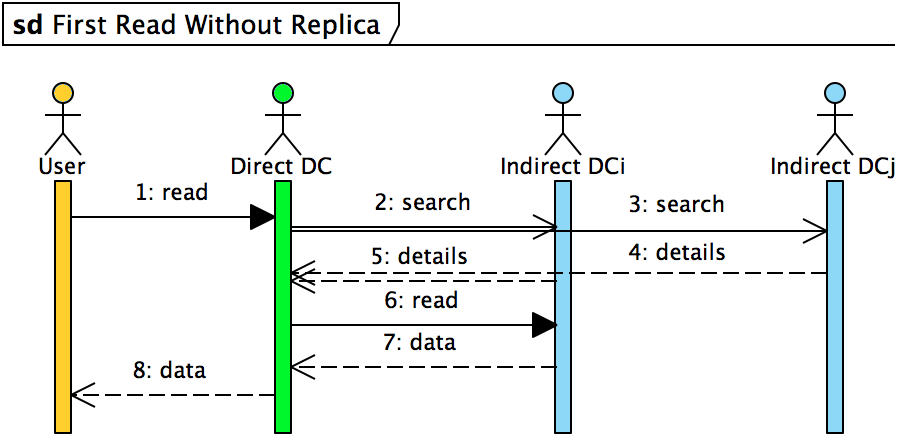
\includegraphics[width=1\textwidth]{figures/firstReadWithoutReplica.png} \\
			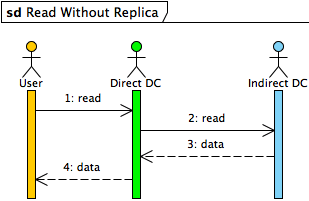
\includegraphics[width=.7\textwidth]{figures/readWithoutReplica.png} \\
			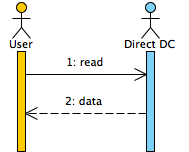
\includegraphics[width=.45\textwidth]{figures/readWithReplica.png}
		\end{tabular}
		
		\caption{Read Sequence Diagrams.}
		\label{tb:read_sequence_diagrams}
	\end{center}
\end{table}
\begin{figure}[ht!]
	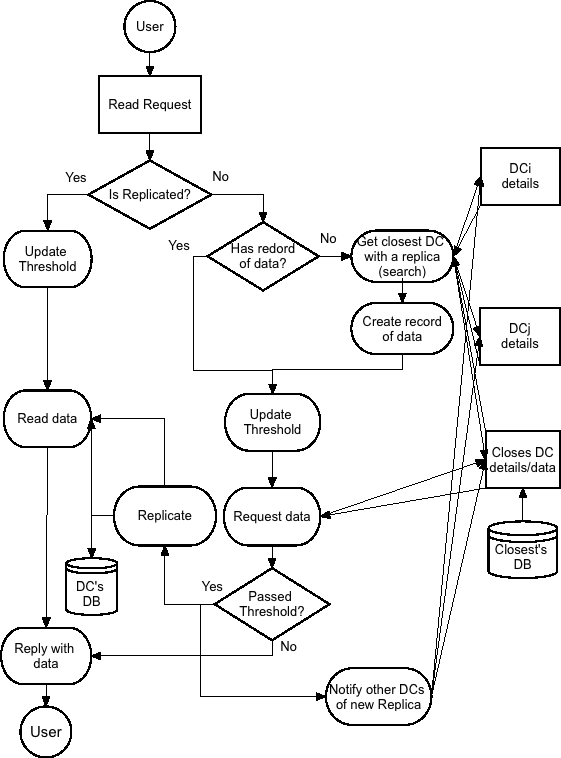
\includegraphics[width=1\textwidth]{figures/readRequestFlowchart.png}

	\caption{Flowchart for read requests.}
	\label{fig:read_flowchart}
\end{figure}

\begin{table}[ht!]
	\begin{center}
		\begin{tabular}{c}
			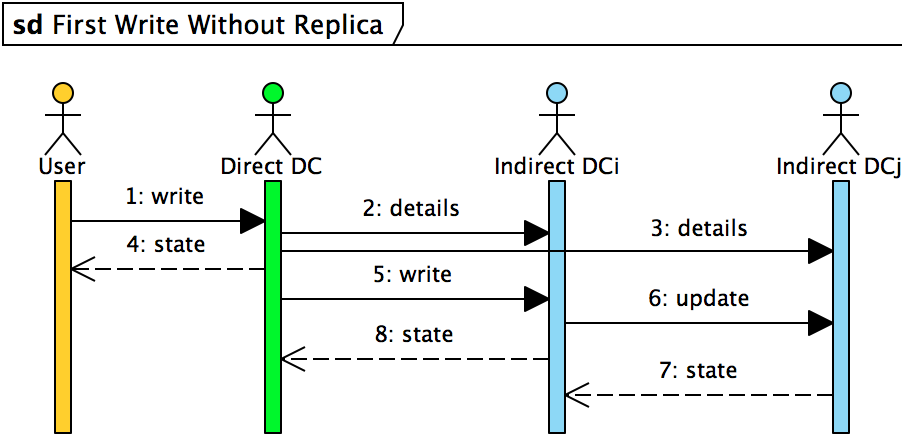
\includegraphics[width=1\textwidth]{figures/firstWriteWithoutReplica.png} \\
			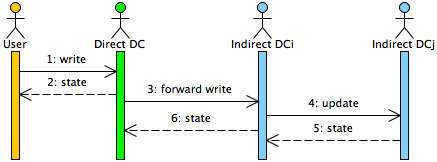
\includegraphics[width=1\textwidth]{figures/writeWithoutReplica.png} \\
			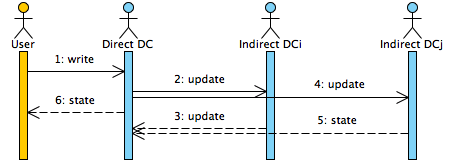
\includegraphics[width=1\textwidth]{figures/writeWithReplica.png}
		\end{tabular}
		
		\caption{Write Sequence Diagrams.}
		\label{tb:write_sequence_diagrams}
	\end{center}
\end{table}
\begin{figure}[ht!]
	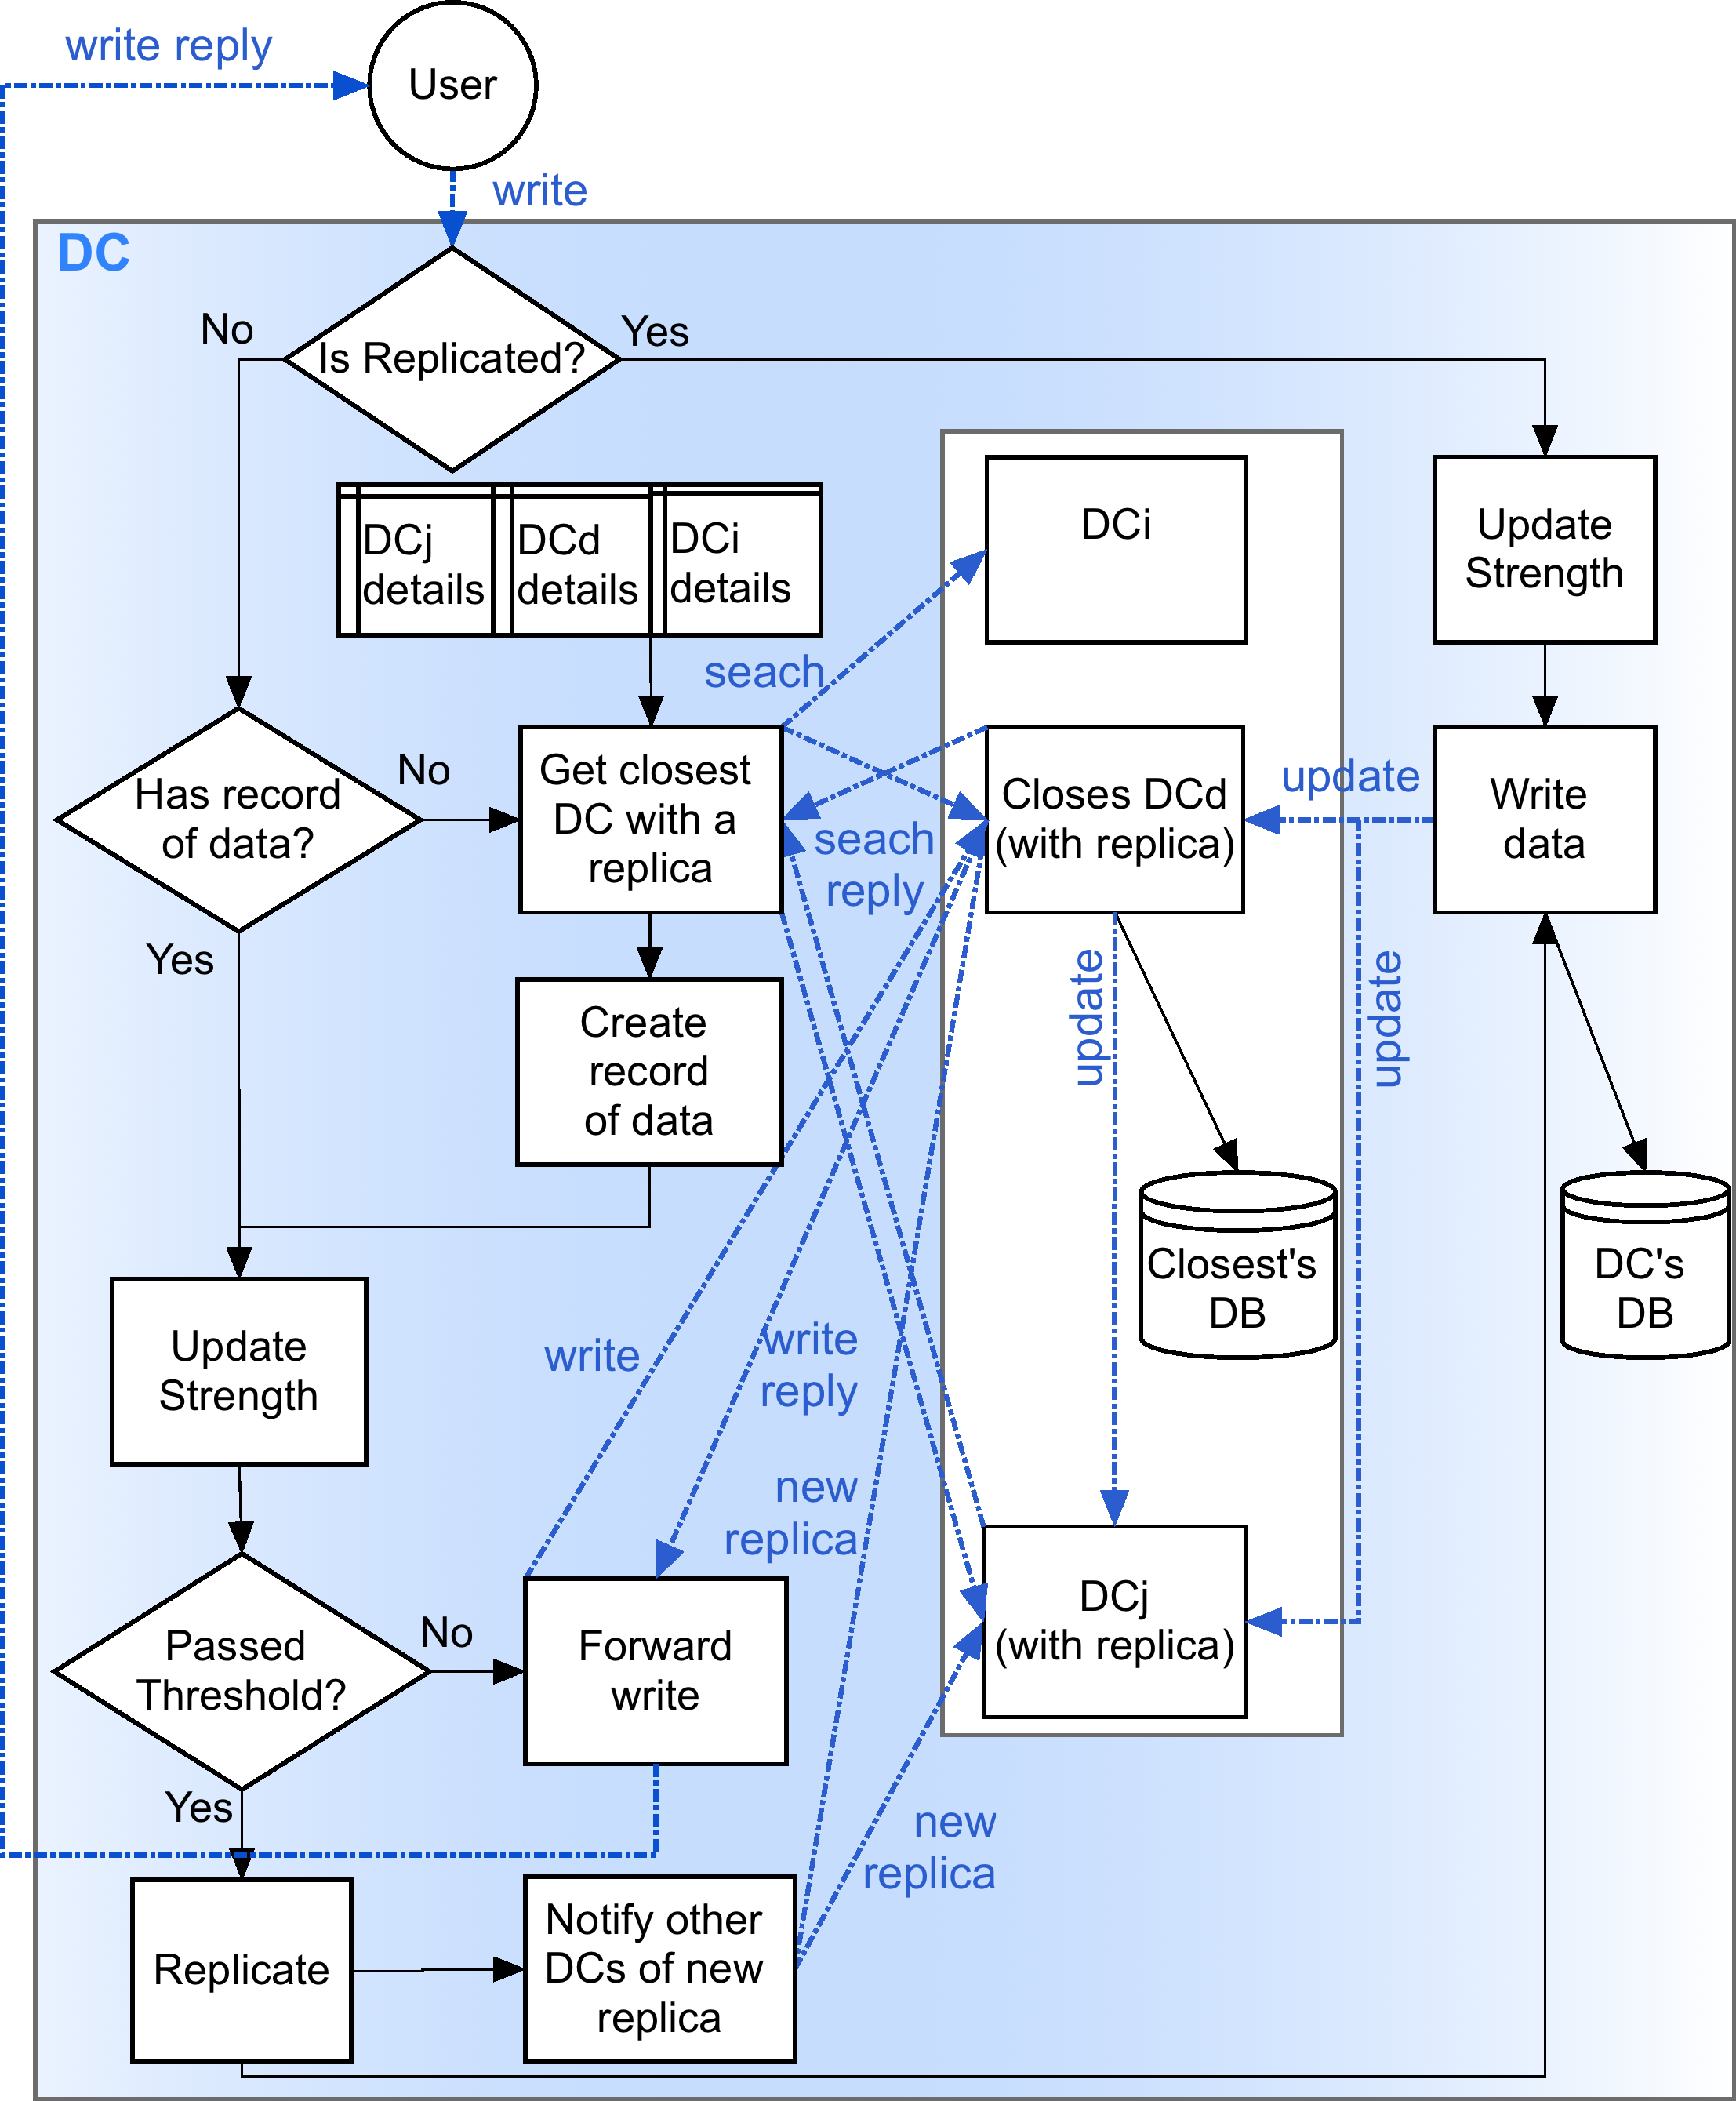
\includegraphics[width=1\textwidth]{figures/writeRequestFlowchart.png}
	
	\caption{Flowchart for write requests.}
	\label{fig:write_flowchart}
\end{figure}

{\bf Some notes on parameters}: 

Given that the number of read is expected to be higher than the number of writes, and normally a read will be executed before a write, it may make sense for $\Delta w_{k}$ to be smaller than $\Delta r_{k}$ ($\Delta w_{k} < \Delta r_{k}$) so that more writes would be required to maintain or create a replica in a \gls{dc} than when using reads.

Some of the parameters may be generalised even further by allowing them to depend on the \gls{dc} the calculation executed in, e.g. $\Delta r_{kd}$ instead of $\Delta r_{k}$ and $\Delta w_{kd}$ instead of $\Delta w_{k}$. Even the terms $r_{k} * \Delta r_{k}$ and $w_{k} * \Delta w_{k}$ could be generalise to consider other factors like bandwidth use and current storage capacity available in the \gls{dc}, or new terms could be added to take account of those new factors.

\section{Summary}
This algorithm implies:
\begin{enumerate}
	\item For reads on a \gls{dc}, the \gls{dc} does not require to communicate any information to any of the other \glspl{dc}. A read only needs to use resources in the \gls{dc}, where the read is initially requested from, so no extra network traffic is imposed on the systems.
	
	In the particular case where a read is executed on a \gls{dc}, without a replica of the data, storage and processing power in the \gls{dc} will be required and the request will be to forwarded the request to its closest \gls{dc} with a replica. This operation incurs in extra network traffic but if it is repeated too often the extra network traffic will be removed by replicating the data in the requesting \gls{dc}.
	
	\item On a write  the \gls{dc} receiving the original request will (eventually) transmit it to the other \glspl{dc}, which have a replica of the data, so no need to add extra network traffic as this is the normal approach. But extra data will be sent to the other \glspl{dc} to notify them of the number of writes the changes refer to, which will depend of the type of \gls{crdt} approach used, i.e. op-based or state-based. In some cases not every write is transmitted to the other \glspl{dc}, such is the case of the state-base approach, so it would be required to keep some track of the number of merged writes.
	
	Also the merging the data should only be executed after the replication strength has been calculating and it is still higher than zero, which will reduce unnecessary operations.

	\item On data without reads and writes concentrated on one \gls{dc}, the number of replicas will be reduced as time passes by the temporal effect ($\Gamma$), until the data is only replicated in one \gls{dc}.
\end{enumerate}

This approach requires simple and fast operations to adapt to the changing conditions of the accessed data.


\section{Acknowledgements}
This work is part of the European research project \href{https://syncfree.lip6.fr}{SyncFree}.


%
% The following two commands are all you need in the initial runs of your .tex file to produce the bibliography for the citations in your paper.
\bibliographystyle{plainnat}
%\bibliographystyle{natbib}
%\bibliographystyle{abbrv}
\bibliography{../syncFree}
% You must have a proper ".bib" file and remember to run:
% latex bibtex latex latex to resolve all references

\printglossaries
\end{document}
